\subsection*{ГЛ12 6}
\begin{figure}[h!]
	\center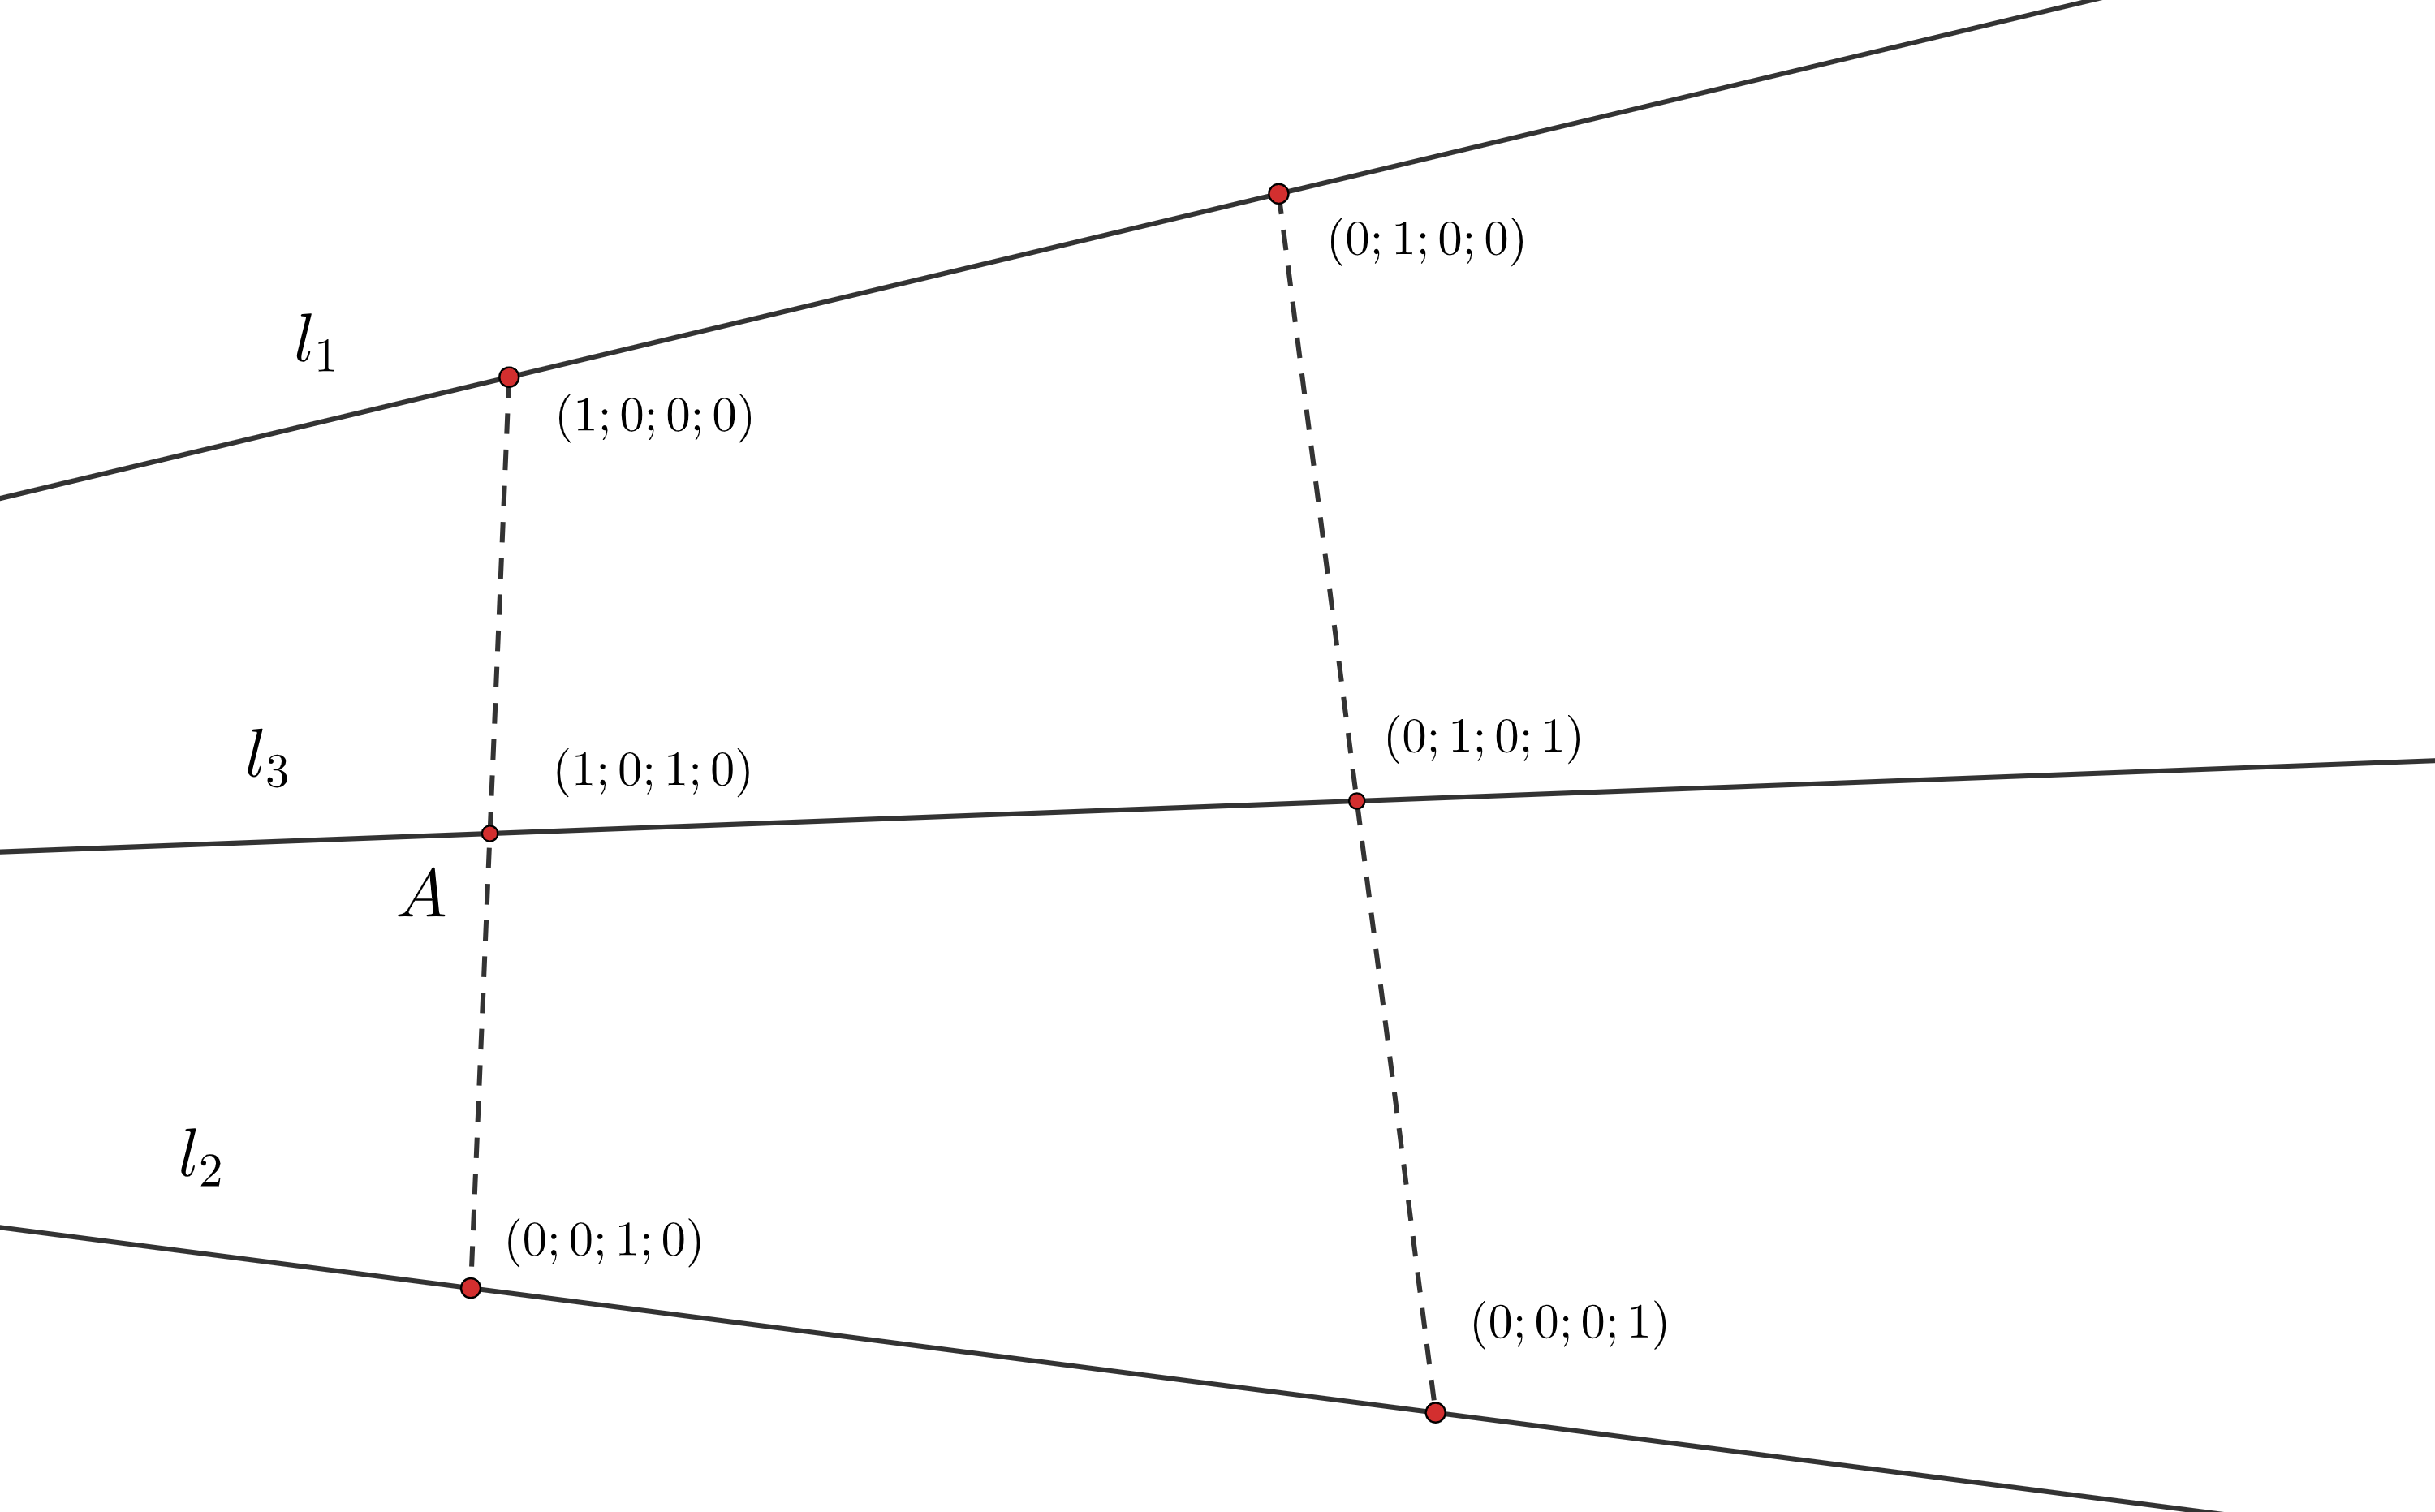
\includegraphics[width=0.4\linewidth]{pic27}
\end{figure}
Пусть $A \in l_3$, где $l_3 = (xyxy)$.\\
$S_1$ -- плоскость, проходящая через $A$ и $l_1$, а $S_2$ -- плоскость, проходящая через $A$ и $l_2$. $S_1 \cap S_2 = L$ -- прямая, $A \in L$, следовательно, существует единственная прямая, пересекающая $l_1, l_2$ и проходящая через $A$. 
\vskip 0.2in
\noindent
Пусть $p_1 = (\alpha : \beta : 0 : 0), p_2 = (0 : 0 : \gamma : \delta)$. Тогда $p_1p_2 \cap l_3 \rightarrow (\mu\alpha : \mu\beta : \lambda\gamma : \lambda\delta) = (x : y : x : y)$, следовательно $\alpha : \beta = \gamma : \delta$\\
\noindent
Множество таких прямых -- это квадрика $Q = x_0x_3 - x_1x_2 = 0$ \\
\noindent
На самом деле, $l_3$ устанавливает проективное соответствие между $l_1$ и $l_2$.\\
Когда и прямые: $l_3: l_2 \rightarrow l_1, \ \ l_4: l_2 \rightarrow l_1$.\\
Тогда искомые прямые $l_3(t_0) = l_4(t_0)$, которых может быть $0, 1, 2, \infty$
\vskip 0.2in
\noindent
$0$ прямых не может быть в $\mathbb{C}^2$, $1$ прямая может быть, но она неустойчива к малым шевелениям, $2$ прямые могут быть и они устойчивы к малым шевелениям.

